\documentclass[12pt,letterpaper]{article}
\usepackage{graphicx,textcomp}
\usepackage{natbib}
\usepackage{setspace}
\usepackage{fullpage}
\usepackage{color}
\usepackage[reqno]{amsmath}
\usepackage{amsthm}
\usepackage{fancyvrb}
\usepackage{amssymb,enumerate}
\usepackage[all]{xy}
\usepackage{endnotes}
\usepackage{lscape}
\newtheorem{com}{Comment}
\usepackage{float}
\usepackage{hyperref}
\newtheorem{lem} {Lemma}
\newtheorem{prop}{Proposition}
\newtheorem{thm}{Theorem}
\newtheorem{defn}{Definition}
\newtheorem{cor}{Corollary}
\newtheorem{obs}{Observation}
\usepackage[compact]{titlesec}
\usepackage{dcolumn}
\usepackage{tikz}
\usetikzlibrary{arrows}
\usepackage{multirow}
\usepackage{xcolor}
\newcolumntype{.}{D{.}{.}{-1}}
\newcolumntype{d}[1]{D{.}{.}{#1}}
\definecolor{light-gray}{gray}{0.65}
\usepackage{url}
\usepackage{listings}
\usepackage{color}

\definecolor{codegreen}{rgb}{0,0.6,0}
\definecolor{codegray}{rgb}{0.5,0.5,0.5}
\definecolor{codepurple}{rgb}{0.58,0,0.82}
\definecolor{backcolour}{rgb}{0.95,0.95,0.92}

\lstdefinestyle{mystyle}{
	backgroundcolor=\color{backcolour},   
	commentstyle=\color{codegreen},
	keywordstyle=\color{magenta},
	numberstyle=\tiny\color{codegray},
	stringstyle=\color{codepurple},
	basicstyle=\footnotesize,
	breakatwhitespace=false,         
	breaklines=true,                 
	captionpos=b,                    
	keepspaces=true,                 
	numbers=left,                    
	numbersep=5pt,                  
	showspaces=false,                
	showstringspaces=false,
	showtabs=false,                  
	tabsize=2
}
\lstset{style=mystyle}
\newcommand{\Sref}[1]{Section~\ref{#1}}
\newtheorem{hyp}{Hypothesis}

\title{Problem Set 2}
\date{Due: October 22, 2026}
\author{Samantha Richter, Applied Stats/Quant Methods 1}

\begin{document}
	\maketitle
	\section*{Instructions}
\begin{itemize}
	\item Please show your work! You may lose points by simply writing in the answer. If the problem requires you to execute commands in \texttt{R}, please include the code you used to get your answers. Please also include the \texttt{.R} file that contains your code. If you are not sure if work needs to be shown for a particular problem, please ask.
	\item Your homework should be submitted electronically on GitHub.
	\item This problem set is due before 23:59 on Thursday October 22, 2026. No late assignments will be accepted.

\end{itemize}

	
	\vspace{.5cm}
	\section*{Question 1: Political Science}
		\vspace{.25cm}
	The following table was created using the data from a study run in a major Latin American city.\footnote{Fried, Lagunes, and Venkataramani (2010). ``Corruption and Inequality at the Crossroad: A Multimethod Study of Bribery and Discrimination in Latin America. \textit{Latin American Research Review}. 45 (1): 76-97.} As part of the experimental treatment in the study, one employee of the research team was chosen to make illegal left turns across traffic to draw the attention of the police officers on shift. Two employee drivers were upper class, two were lower class drivers, and the identity of the driver was randomly assigned per encounter. The researchers were interested in whether officers were more or less likely to solicit a bribe from drivers depending on their class (officers use phrases like, ``We can solve this the easy way'' to draw a bribe). The table below shows the resulting data.

\newpage
\begin{table}[h!]
	\centering
	\begin{tabular}{l | c c c }
		& Not Stopped & Bribe requested & Stopped/given warning \\
		\\[-1.8ex] 
		\hline \\[-1.8ex]
		Upper class & 14 & 6 & 7 \\
		Lower class & 7 & 7 & 1 \\
		\hline
	\end{tabular}
\end{table}

\begin{enumerate}
	
	\item [(a)]
	Calculate the $\chi^2$ test statistic by hand/manually (even better if you can do "by hand" in \texttt{R}).\\
	\lstinputlisting[language=R, firstline=39, lastline=97]{PS02.R}
	\noindent \textbf{Answer:} The $\chi^2$ test statistic is $\chi^2 = 3.79$, with 2 degrees of freedom.
	\noindent A chi-squared ($\chi^2$) test of independence tells me whether two categorical variables (1) driver class (upper or lower) and 2) police behavior are associated with each other. My null hypothesis is $H_0$: Driver class and police officer behavior are statistically independent (there is no association between driver class and police behavior). My alternative hypothesis is $H_A$: Driver class and police officer behavior are not statistically independent (there is an association between driver class and police officers’ behavior).
	\noindent The chi-squared test compares observed counts ($f_o$) to expected counts($f_e$) if $H_0$ were true. The bigger the gaps between them, the more evidence there is against satistical independence between x and y. 
	
	\noindent \textit{Step 1: Marginal totals.} To figure out the expected counts, I need the marginal total for each row and column to see how each variable is distributed on its own. 
	
	\noindent \textit{Step 2: Find expected frequencies.} If the driver class and police behavior were independent of each other, each behavior should happen at the same rate for upper and lower classes. The expected count for each cell is: \[ f_e = \frac{\text{row total} \times \text{column total}}{n} \]  
	\begin{table}[H]
		\centering
		\begin{tabular}{l | c c c }
			Expected ($f_e$) & Not Stopped & Bribe requested & Stopped/given warning \\
			\\[-1.8ex] 
			\hline \\[-1.8ex]
			Upper class & 13.50 & 8.36 & 5.14 \\
			Lower class & 7.50 & 4.64 & 2.86 \\
			\hline
		\end{tabular}
	\end{table}
	\noindent \textit{Step 3: Calc test statistic.} The $\chi^2$ statistic adds the squared difference between the observed and expected counts across all six cells, divided by expected count: \[ \chi^2 = \sum \frac{(f_o - f_e)^2}{f_e} \] We square the difference so that positive and negative gaps don’t cancel out. Dividing by $f_e$ makes each difference standardized to the cell size. 
	\begin{table}[H]
		\centering
		\begin{tabular}{l | c c c }
		    Contribution & Not Stopped & Bribe requested & Stopped/given warning \\
			\\[-1.8ex] 
			\hline \\[-1.8ex]
			Upper class & 0.02 & 0.66 & 0.67 \\
			Lower class & 0.03 & 1.20 & 1.21 \\
			\hline
		\end{tabular}
	\end{table}
	\noindent Summing these equals $\chi^2 = 3.79$. The built-in \texttt{chisq.test()} function shows the same result. Most of chi-squared comes from the bribe requested and stopped/given warning columns, especially for lower class drivers. The not stopped column contributes almost nothing to the statistic. This means that drivers of lower and upper classes were not stopped at about the rate we’d expect under independence (H0). 
	
	\item [(b)]
	Now calculate the p-value from the test statistic you just created (in \texttt{R}).\footnote{Remember frequency should be $>$ 5 for all cells, but let's calculate the p-value here anyway.}  What do you conclude if $\alpha = 0.1$?\\
	\lstinputlisting[language=R, firstline=99, lastline=118]{PS02.R}
	\noindent \textbf{Answer:}  P-value = 0.150. Since this is greater than $\alpha = 0.1$, I fail to reject the null hypothesis. From the evidence, I can't conclude that driver class and police behavior are associated (statistically dependent) in the population.
	\noindent The p-value is the probability of getting a $\chi^2$ statistic at least as large as 3.79 if the $H_0$ (unrelated class and police behavior) was true. A small p-value means that the data would be unlikely under $H_0$. For p-value in chi-squared, we must include the degrees of freedom, because the shape of the chi-squared distribution depends on them: \[ df = (\text{rows} - 1) \times (\text{columns} - 1) = (2 - 1) \times (3 - 1) = 2 \] The p-value is the area to the right of 3.79 under the distribution shape with 2 degrees of freedom, since we only looked at the upper tail (only large differences between observed and expected count as evidence against $H_0$). The built-in \texttt{chisq.test()} function gives the same p-value. This doesn't prove that police treat upper and lower class drivers the same, but it shows that this data doesn't give strong enough evidence of an association (statistical dependence). 
	\newpage
	\item [(c)] Calculate the standardized residuals for each cell and put them in the table below.
	\lstinputlisting[language=R, firstline=120, lastline=146]{PS02.R}
	\begin{table}[h]
		\centering
		\begin{tabular}{l | c c c }
			& Not Stopped & Bribe requested & Stopped/given warning \\
			\\[-1.8ex] 
			\hline \\[-1.8ex]
			Upper class  & 0.32 & -1.64 & 1.52  \\
			\\
			Lower class & -0.32 & 1.64  & -1.52  \\
			
		\end{tabular}
	\end{table}
	\noindent \textbf{Answer:} The standardized residuals measure how far the observed count is from the expected count for each cell, in standard error units. It is calculated as: \[ z = \frac{f_o - f_e}{\sqrt{f_e \, (1 - \text{row proportion}) \, (1 - \text{column proportion})}} \] 
	The row proportion is the row total divided by $n$, and the column proportion is the column total divided by $n$. The built-in \texttt{chisq.test()} function gives the same answers. 
	\noindent The sign gives directionality. A positive cell residual means there were more run-ins than expected under the null hypothesis (independence), and a negative residual means there were less. Since they’re standardized, it’s easier to judge and compare between them. By some standards a value larger than absolute value of 2 (1.96 for $\alpha = 0.05$) or absolute value of 3 indicates a big difference from independence in that cell. \noindent In this case, the rows are opposites (in terms of sign). This is because with only two rows, if one class has more encounters than expected in a column, the other class must have fewer.
	
	\item [(d)] How might the standardized residuals help you interpret the results?  
	
	\noindent \textbf{Answer:} The standardized residuals show which cells contribute most to the overall chi squared result, and their sign shows the direction (positive means more than we'd expect under independence, negative means fewer). This gives more detail than the single $\chi^2$ statistic, which tells us whether variables overall are dependent or not.
	
	\noindent Looking at the frequency table, there is no strong pattern between driver class and policy behavior, and the standardized residuals support this since they are all small. The largest is for bribe requested ($\pm 1.64$), where lower class drivers were asked for a bribe a bit more often than we'd expect under independence (7 observed vs. 4.64 expected) and upper class drivers a bit less often (6 vs. 8.36). For not stopped ($\pm 0.32$), the residual is very close to 0, so drivers of both classes were not stopped at almost exactly the rate we'd expect under independence. 
	
	\noindent However, no cell is significantly different from what we'd expect under independence at the 0.05 level. This matches my result in part (b), where I failed to reject the null.  
\end{enumerate}
\newpage

\section*{Question 2: Economics}
Chattopadhyay and Duflo were interested in whether women promote different policies than men.\footnote{Chattopadhyay and Duflo. (2004). ``Women as Policy Makers: Evidence from a Randomized Policy Experiment in India. \textit{Econometrica}. 72 (5), 1409-1443.} Answering this question with observational data is pretty difficult due to potential confounding problems (e.g. the districts that choose female politicians are likely to systematically differ in other aspects too). Hence, they exploit a randomized policy experiment in India, where since the mid-1990s, $\frac{1}{3}$ of village council heads have been randomly reserved for women. A subset of the data from West Bengal can be found at the following link: \url{https://raw.githubusercontent.com/kosukeimai/qss/master/PREDICTION/women.csv}\\

\noindent Each observation in the data set represents a village and there are two villages associated with one GP (i.e. a level of government is called "GP"). Figure~\ref{fig:women_desc} below shows the names and descriptions of the variables in the dataset. The authors hypothesize that female politicians are more likely to support policies female voters want. Researchers found that more women complain about the quality of drinking water than men. You need to estimate the effect of the reservation policy on the number of new or repaired drinking water facilities in the villages.
\begin{figure}[h!]
	\caption{\footnotesize{Names and description of variables from Chattopadhyay and Duflo (2004).}}
	\vspace{.5cm}
	\centering
	\label{fig:women_desc}
	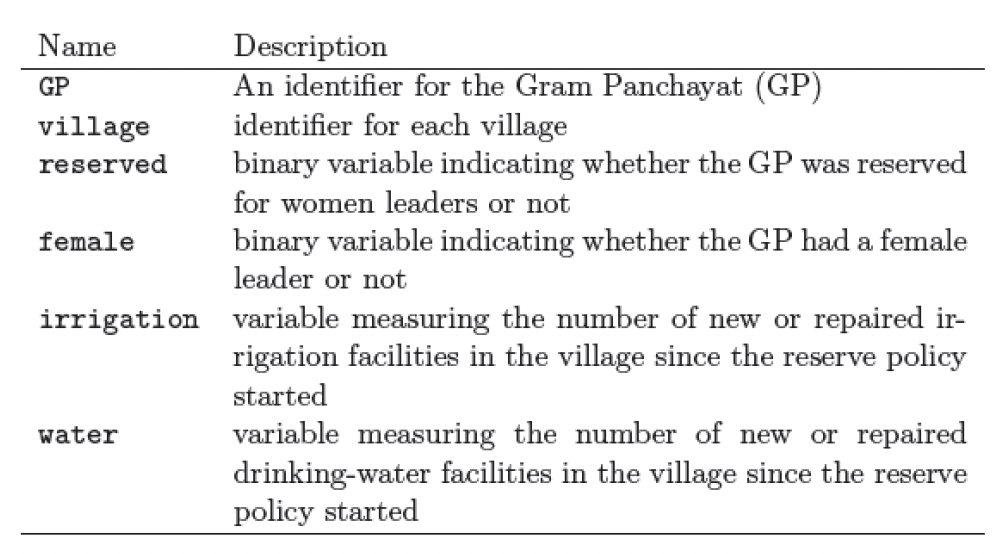
\includegraphics[width=1.1\textwidth]{women_desc.png}
\end{figure}		

\newpage
\begin{enumerate}
	\vspace{1cm}
	\item [(a)] State a null and alternative (two-tailed) hypothesis. 
	\lstinputlisting[language=R, firstline=152, lastline=173]{PS02.R}
	\noindent \textbf{Answer:} \[ H_0: \beta_1 = 0 \qquad H_A: \beta_1 \neq 0 \] 
	
	\noindent The regression model: \[ \text{water} = \beta_0 + \beta_1 \, \text{reserved} + \epsilon \] is used to test the effect of the reservation policy. Water is the number of new or repaired drinking facilities in a village, and Reserved = 1 if the village's GP was reserved for a woman and 0 if not. Because that’s only two values, $\beta_1$ is the difference in the average number of drinking facilities between the two types of villages. 
	
	$H_0$: $\beta_1 = 0$. The reservation policy has no effect on the number of new or repaired drinking-water facilities. On average, reserved and unreserved villages have the same number of facilities in the population.
	$H_A$: $\beta_1 \neq 0$. The reservation policy has some effect on the number of new or repaired drinking-water facilities, in either direction (two-tailed). On average, reserved and unreserved villages have a different number of facilities in the population.
	
	The authors expect female leaders to invest more in drinking water, which would suggest they expect Ha to be greater than 0. 
	
	I chose reserved as the explanatory variable because it was randomly assigned and shows the effect of that policy on drinking water. Before writing the hypotheses, I checked the data and saw that about a third of villages (total = 322) have reserved GPs, which matches the policy design.
	
	\vspace{1cm}
	\item [(b)] Run a bivariate regression to test this hypothesis in \texttt{R} (include your code!).
	\lstinputlisting[language=R, firstline=175, lastline=194]{PS02.R}
	\noindent \textbf{Answer:} The coefficient for the slope is $\hat{\beta}_1 = 9.25$, with a p-value of 0.020. Since this is below $\alpha = 0.05$, I can reject the null hypothesis that the reservation policy has no effect on the number of new or repaired drinking facilities. 
	\noindent A bivariate regression shows the outcome variable of water as a linear function of the reserved variable. Using summary() to look at the estimated coefficients:
\begin{verbatim}
	Coefficients:
	Estimate Std. Error t value Pr(>|t|)    
	(Intercept)   14.738      2.286   6.446 4.22e-10 ***
	reserved       9.252      3.948   2.344   0.0197 *  
	---
	Signif. codes:  0 ‘***’ 0.001 ‘**’ 0.01 ‘*’ 0.05 ‘.’ 0.1 ‘ ’ 1
	
	Residual standard error: 33.45 on 320 degrees of freedom
	Multiple R-squared:  0.01688,	Adjusted R-squared:  0.0138 
	F-statistic: 5.493 on 1 and 320 DF,  p-value: 0.0197
\end{verbatim}
	\noindent The test statistic shows how many standard errors the estimate is away from 0. The degrees of freedom are $n - 2 = 322 - 2 = 320$, because the model estimates ($\beta_0$ and $\beta_1$). Because the test is two-tailed, the p-value includes the area in both tails.
	
	\noindent Since $p = 0.020 < 0.05$, I can reject $H_0$. 
	
	\item [(c)] Interpret the coefficient estimate for reservation policy. 
	
	\noindent \textbf{Answer:} The coefficient estimate of 9.25 means that villages in GPs reserved for women were associated with, on average, about 9.25 more new or repaired drinking-water facilities than unreserved villages. 
	
	\noindent Unreserved villages had 14.74 facilities on average. Reserved villages had 14.74 + 9.25 = 23.99 facilities on average. So the coefficient $\beta_1$ is just the difference between the two group averages. This difference is statistically significant at $\alpha = 0.05$ with ($p = 0.020$). 
	
	\noindent The result supports that GPs reserved for women leaders invested more in drinking water. However, I would not draw a causal conclusion due to some limitations: large relative standard errors (and Confidence Intervals); there are village outliers, including one with 340, which regression estimates are sensitive to, and other unknown factors of the research.

\end{enumerate}


%\end{enumerate}
\end{document}
